\chapter{Data Discussion and Policy Construction}\label{C:us}

This section addresses the construction of reputation policies for use on Twitter. In particular the development of analysis tools for achieving greater understanding of the Twitter dataset created are discussed, and discussion of hypotheses generated from this data and how we experimented with these. Only Twitter data is discussed due to the richness of the dataset mined. As such multiple analysis approaches were taken.

Data was collected during scraper implementation, as per the feedback loop in figure 5.3. Profiles scraped earlier contain less detail than data collected later. For example, names of retweeters was not a feature collected on earlier profiles. In total, 1767 separate profiles were scraped, totalling 1,745,161 tweets. 

%Twitter data is discussed soley, as the dataset retrieved was rich enough to provide for several analysis angles.
%Fix this

%\section{Collection Method}

%Data discussed was collected entirely from the Twitter Scraper I implemented. This was collected during implementation, as per the feedback loop in figure 5.3. As such, profiles scraped earlier contain less detail than data collected later. 

%Show the median,q1 q3 min max of the number of tweets per profile perhaps?

\section{Retweet Analysis}

Retweets were considered as a basis for policies as more semantic information can be retrieved from retweets than favourites. When retweeting content users are able to comment and add extra value to the post, whereas this is not possible for favourites.

The first question asked was to do with the use of retweet and favourite functionality on Twitter. When \textit{retweeting} content on Twitter, the post will appear on the users own wall, as a tweet. A \textit{favourite} instead is added to a user's list of favourite tweets, which may be viewed separately by other members of Twitter. To demonstrate policy examples later, and to simplify data collection, we put forward that tweets similar in popularity will have equivalent amounts of retweets and favourites. We hypothesise that as a measure of impact, the number of retweets and favourites for an item on Twitter are equivalent.

% \begin{description}
%  \item [H1.]{As a measure of impact, the number of retweets and favourites for an item on Twitter are equivalent.}
% \end{description}

A simple approach to demonstrate that the use of retweets and favourites is equivalent in terms of impact or response is to check the correlation between these figures on a set of tweets. Figure \ref{fig:correlation_retweet_fav} shows this correlation. We find that retweets and favourites have a strong positive correlation, with a Pearson's coefficient r of 0.875 (3.s.f), n = 1,048,576. 

\begin{figure}[h!]
\begin{center}
 \centering
\includegraphics[width=500px]{Images/retweets_vs_favourites.pdf}
\caption{Correlation of Retweet and Favourite Count}
\label{fig:correlation_retweet_fav}
\end{center}
\end{figure}

%Number of tweets compared against
%Correlation

\subsection{Impact Factor}

We created an \textit{impact factor} measurement based upon a Twitter user's retweet count, and tweet activity. This formula is upon the Hirsch-index \cite{hirsch2005index} measurement for an academic's contribution to literature. It attempts to measure both the impact (number of retweets) and productivity (number of tweets) of a Twitter user. 

\begin{figure}[h!]
\begin{center}
\centering
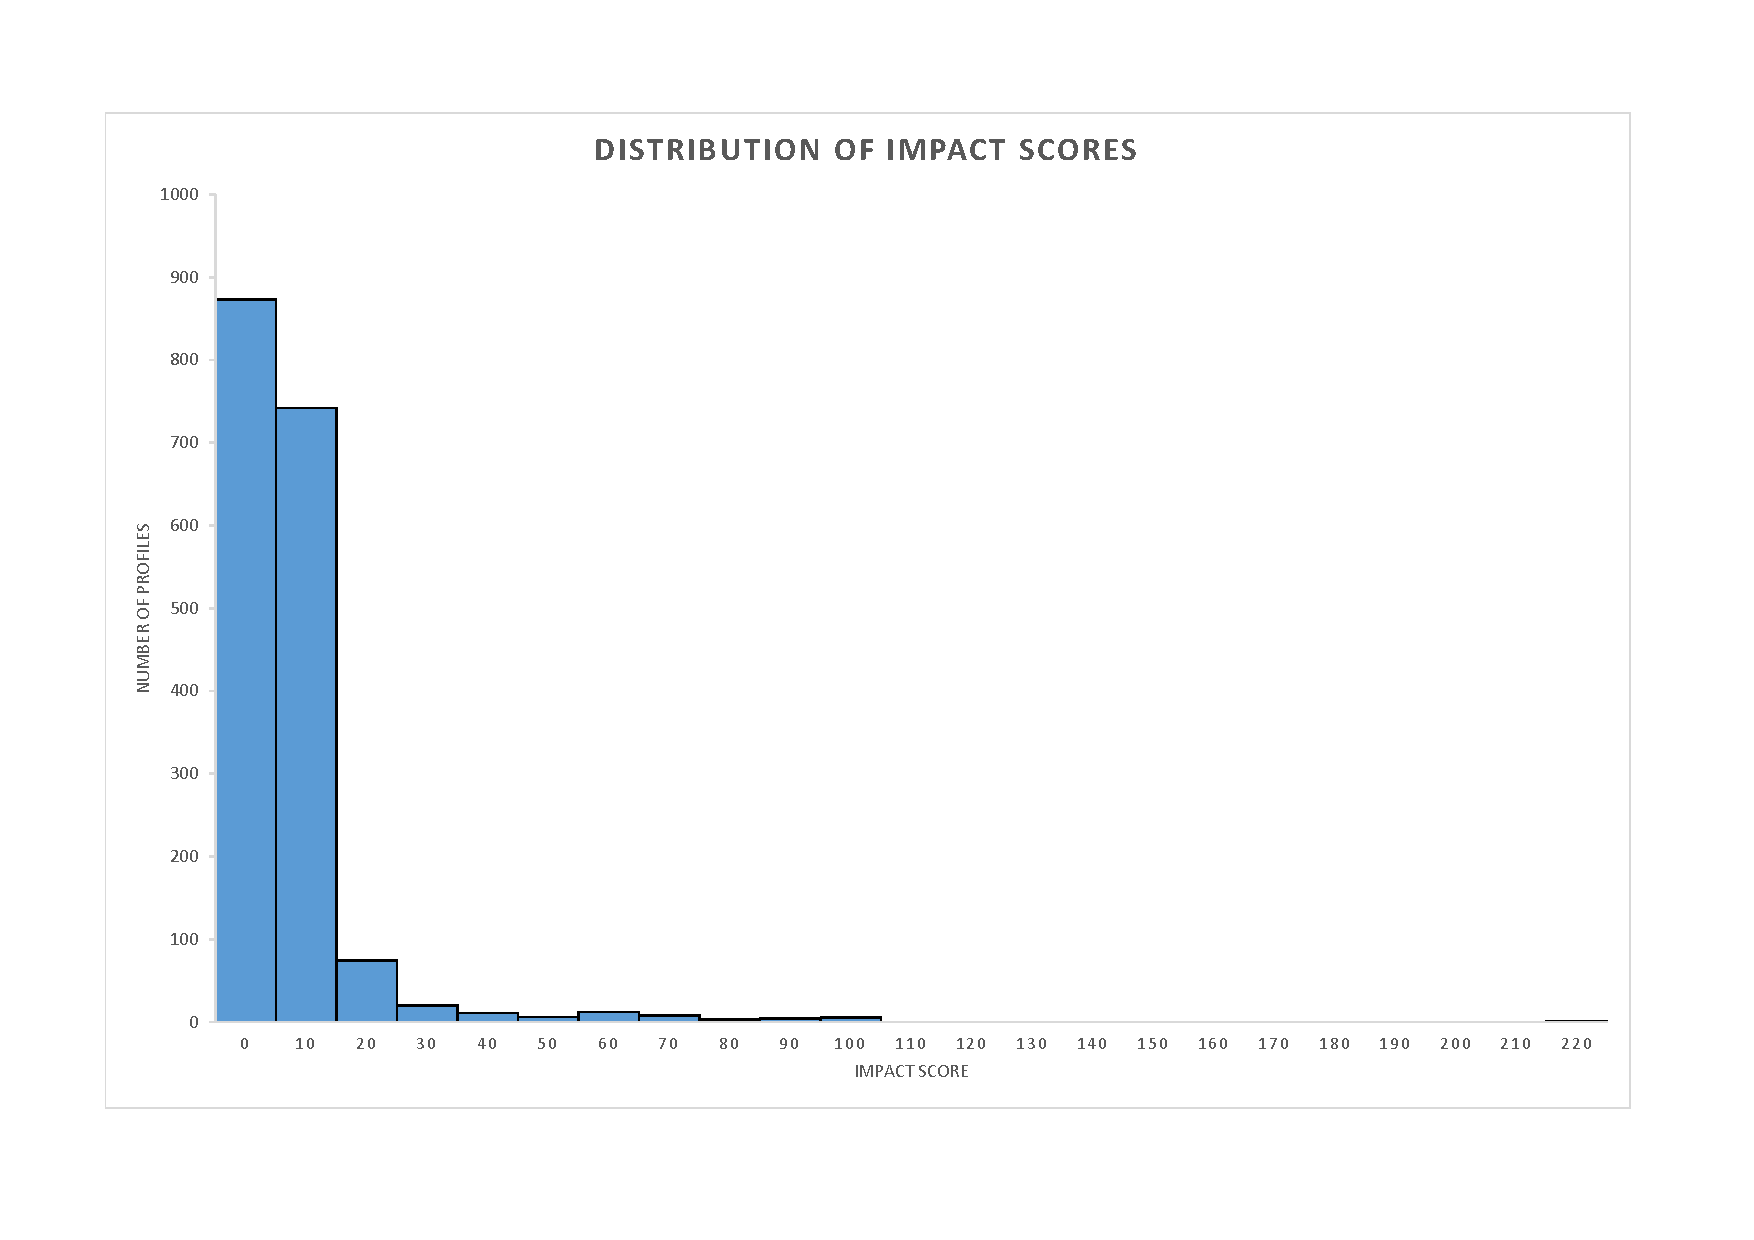
\includegraphics[width=500px]{Images/impact_distribution_histogram.pdf}
\caption{Distribution of Impact Score Among Users}
\label{fig:dist_impact_score}
\end{center}
\end{figure}

Figure \ref{fig:dist_impact_score} displays the distribution of impact factor values, over the set of twitter profiles collected. We can see that the impact score follows a roughly exponentially decreasing curve, with the vast majority of users getting a low impact score. This is reflective of past research, studying the behaviours of Twitter users \cite{beevolve}. That is, user patterns can be broken up into users who follow others and do not post much content themselves, and users who are more active and are followed by others. The extremely high impact scores are likely celebrities - the profile with the highest impact score of 216 was the Jonas Brothers (a pop band) profile, which happened to feature in the dataset. 

The impact factor calculation differs from other social media impact algorithms in that there is no upper limit on score. Other methods are arbitrarily capped at values like 10 or 100, which restricts the comparative value of such tools for the high echelons of impacting-users. The algorithm also automatically takes into account the length of time a user has been active on Twitter when performing the calculation. 

Extensions to the impact factor algorithm could include use of data such as number of followers, as well as frequency or consistency of posting. For example, users which have a large following but whom only have very low retweet counts may imply that content posted is somewhat stale. Also, an individual who had a strong impact in the past but who has not posted recently should logically receive a lower current impact; the current algorithm will not differentiate from an active user and an inactive one. This temporal structuring and analysis for a reputation policy is worth exploring further. 

\subsection{Temporal Clustering and Impact Factor}

In order to differentiate from \textit{one-hit-wonders} and \textit{constant emitters} in reputation policies, some view of activity over time was discussed. We refer to this as temporal clustering. One approach is to cluster impact score calculation into separate months. This reveals how consistently influential a person is, and gives the potential for detecting inactive users. Various bucket sizes were experimented with - days were much to varying to interpret a clear underlying trend, whilst years were too coarse to solve the issue of inactive users receiving a high impact score. Thus months are used as a bucketing measure.

\begin{figure}[h!]
\begin{center}
\centering
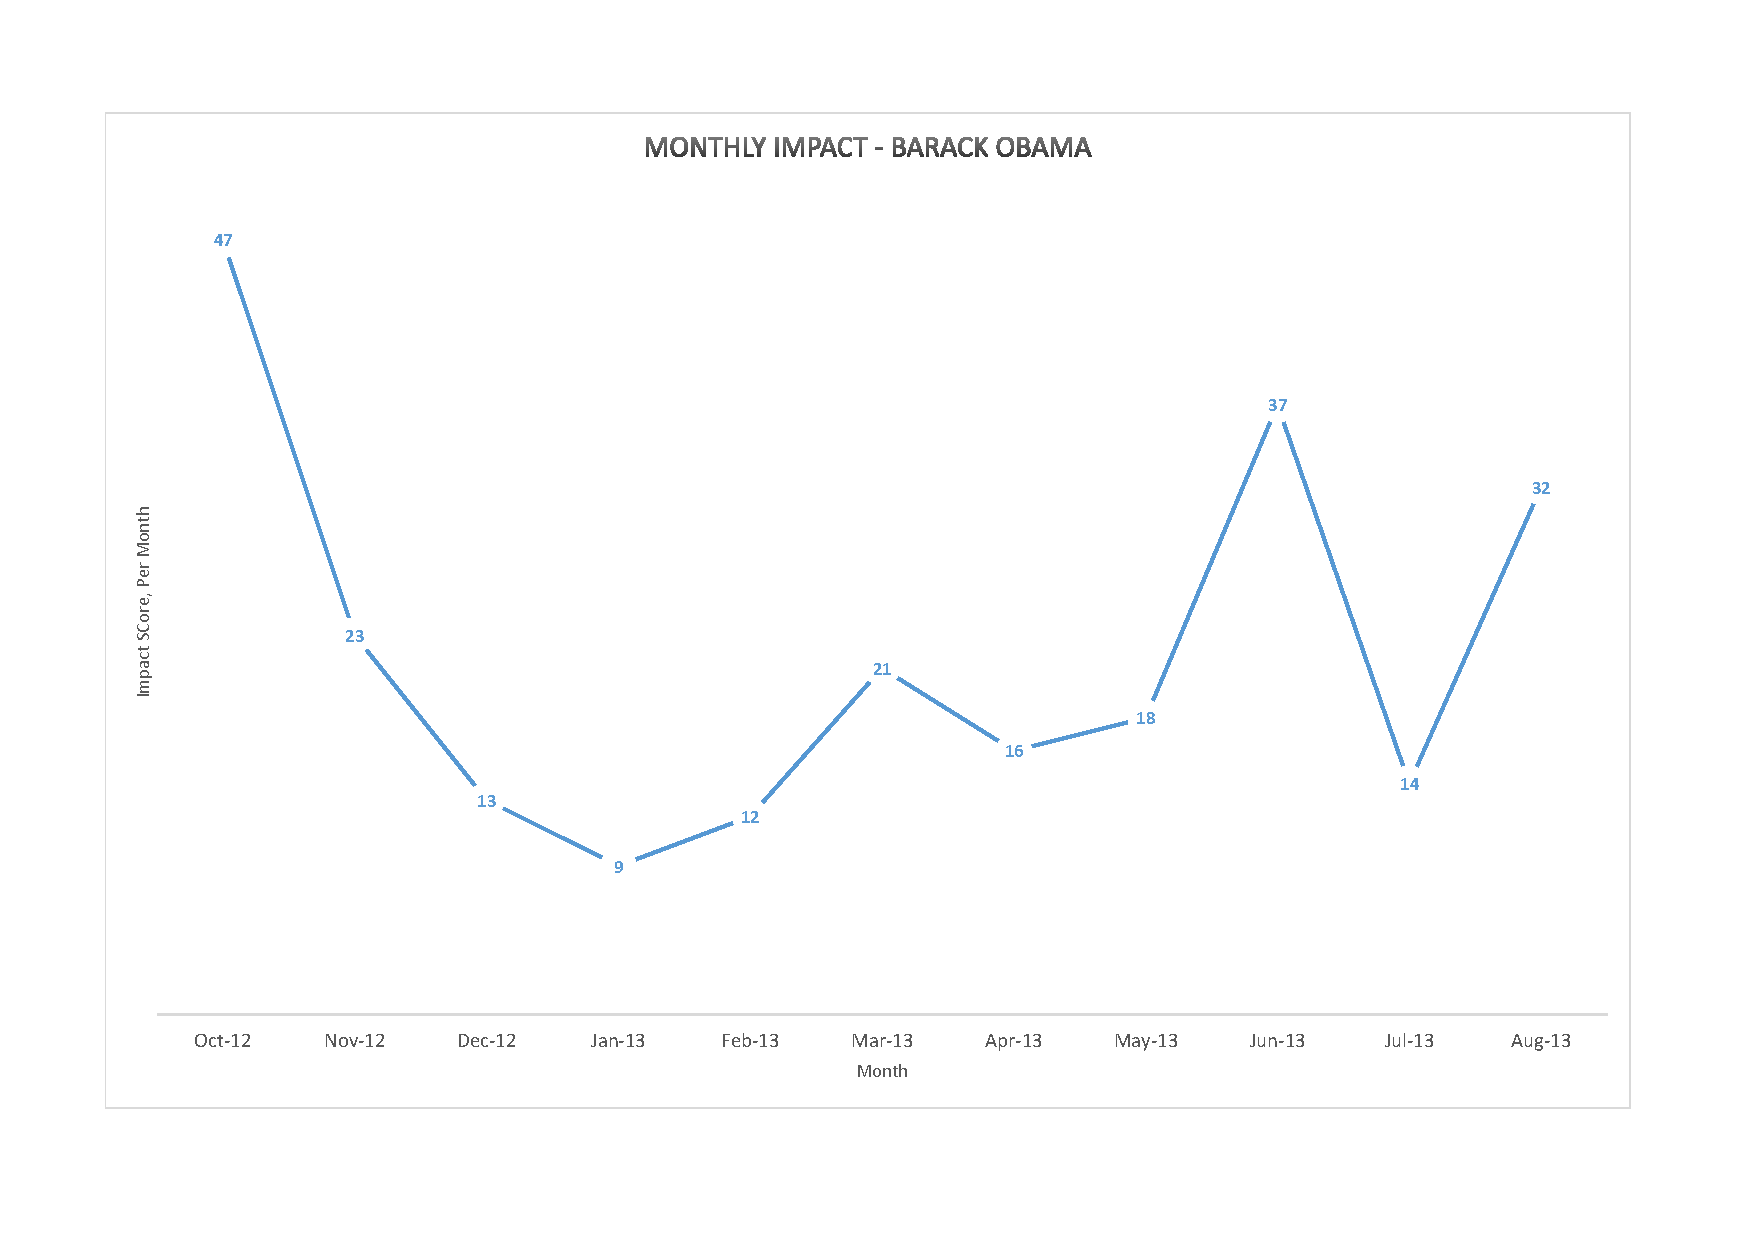
\includegraphics[width=500px]{Images/barack_obama_monthly_impact.pdf}
\caption{An Example of Monthly-Impact Score Bucketing - Barack Obama}
\label{fig:obama}
\end{center}
\end{figure}

This technique can be used to link real-world events to a person's influence. Barack Obama is taken as an example, as seen in Figure \ref{fig:obama}. In October and November of 2012, the US presidential elections were at their peak. The corresponding impact score of 47 for Obama in October is reflective of this. 

To demonstrate this on another individual, take Chris Hadfield (Twitter name Cmdr\_Hadfield), made famous through his cover of David Bowie's 'Space Oddity'. Figure \ref{fig:hadfield} shows how Hadfield's popularity spiked around the time of this video's explosion in popularity - June this year. 

\begin{figure}[h!]
\begin{center}
\centering
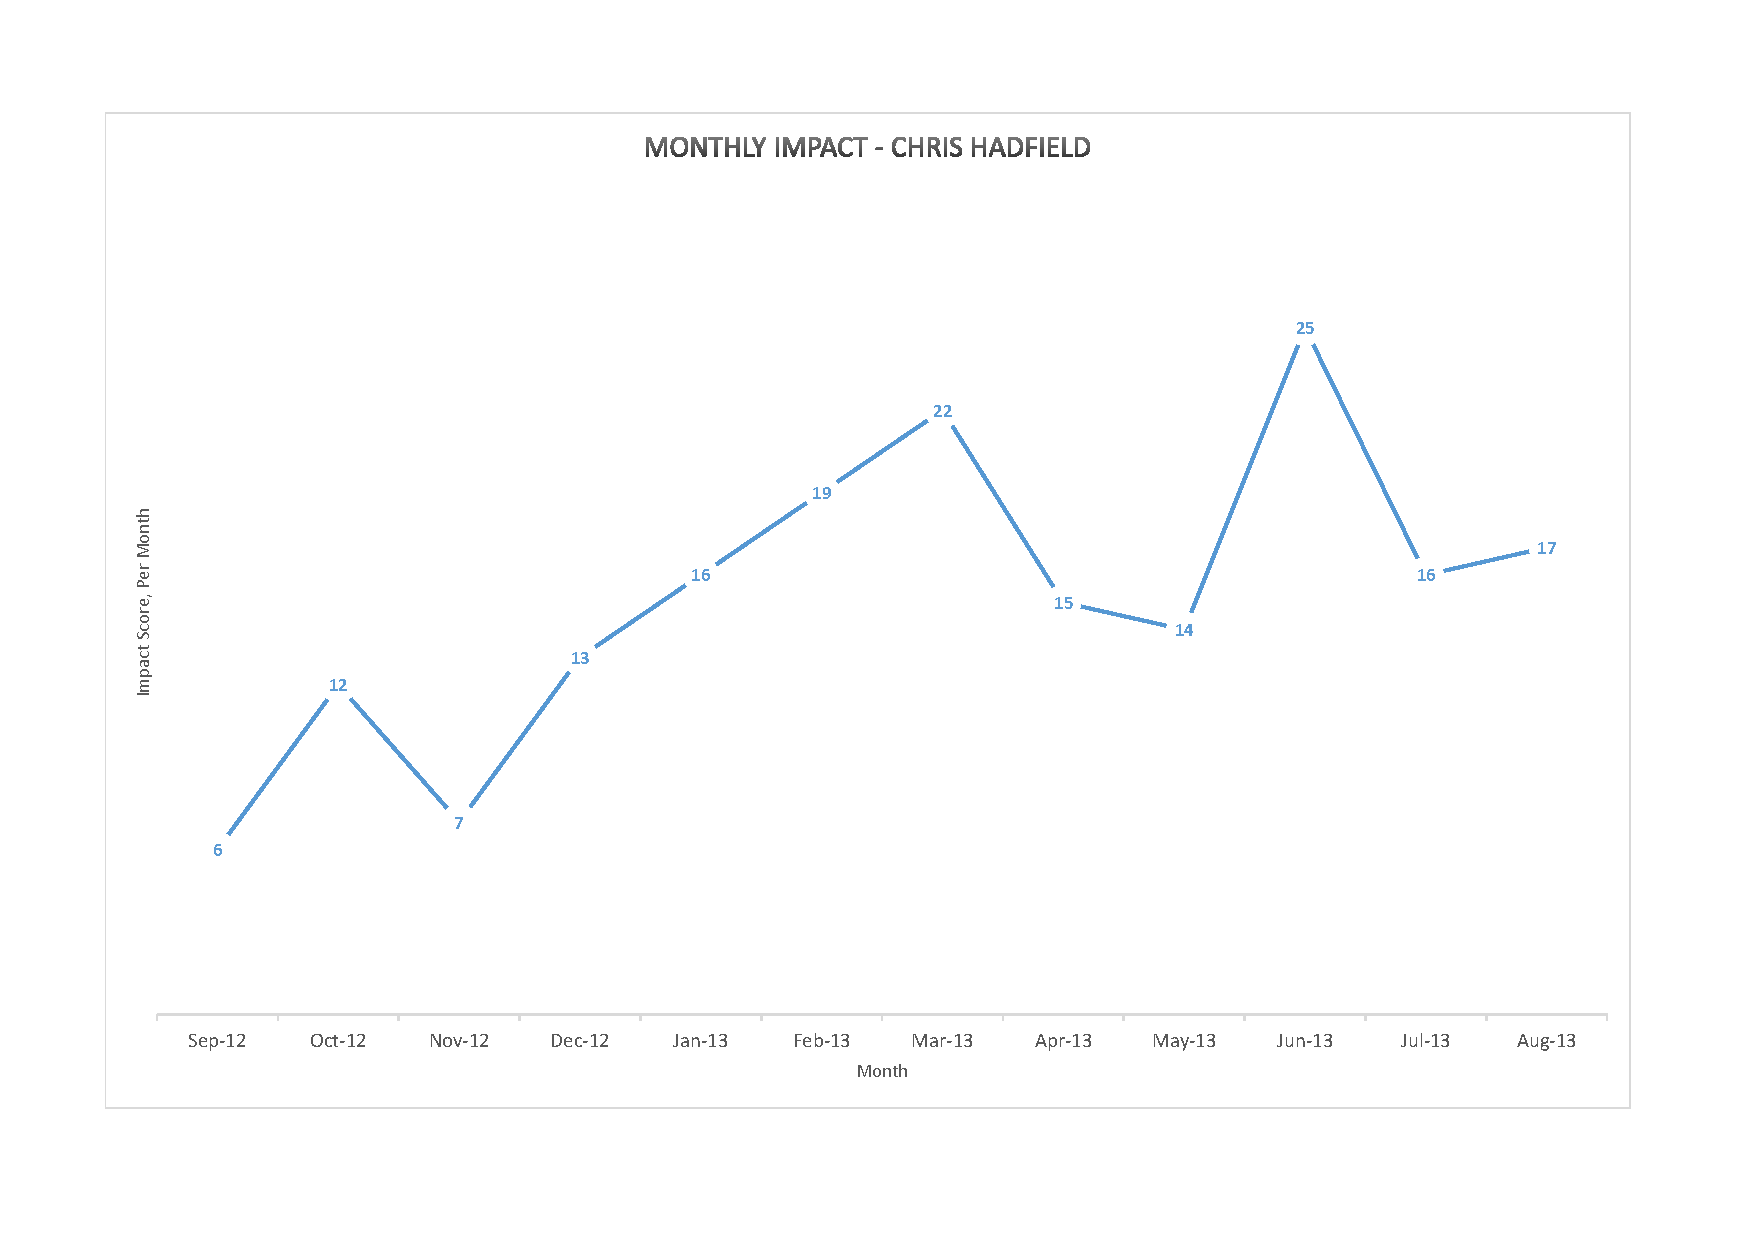
\includegraphics[width=500px]{Images/chris_hadfield_monthly_impact.pdf}
\caption{The Monthly Impact of Chris Hadfield - Famous Astronaut}
\label{fig:hadfield}
\end{center}
\end{figure}

\section{Community Detection}

The second primary data exploration factor explored community detection on Twitter. As a second hypothesis, we attempt to validate that embedded social networks exist within Twitter, and can be detected using IHPScrape. Detection of these communities will be possible through two means; follower and following links, and connection through retweets. Data collected for detecting communities consists of two sets to verify this claim; the retweet links, and follower links. These sets are largely disconnected, and as such discussion of these two techniques must also be separated.  
% 
% I propose the following. 
% 
% \begin{description}
% \item[H2.]{Embedded social networks exist within Twitter, and can be detected using IHPScrape. Detection of these communities will be possible through two means; follower and following links, and connection through retweets.}
% \end{description}



\subsection{MapEquation Tool}

MapEquation is a leading community-detection software tool, which uses graph-traversing techniques to detect the presence of sub-communities in a network \cite{mapequation}. In short, the algorithm aims to cluster neighbouring nodes into modules, then supermodules, and so on. Such an algorithm allows for a good clustering of a network in a very short time, and makes community detection feasible among millions of nodes.

The InfoMap software package distributed by mapequation is compatible with a Flash-based MapGenerator application, also hosted at the MapEquation site \footnote{http://www.mapequation.org/code.html}. This allows communities output through the InfoMap package to be visualised in a sensible manner. The following results were generated by gathering data, running community detection algorithms upon these sets, and visualising the results. Unfortunately the Flash tool is limited in terms of the numbers of nodes which may be loaded. My data consisted of millions of nodes and edges, and often the browser-based applet would cease functioning after data on the order of tens-of-thousands of nodes was loaded. The designers of the application are currently working on a newer version, to allow for larger quantities of data to be loaded through the MapGenerator tool, which would allow for more interesting community analysis in the future. 

\subsection{Followers and Following}

The first community detection approach considers those clustered around profiles, through links in following (profiles an individual is following) and followers (users who are following the current profile). I found that disconnected communities are clustered around popular figures. Figure \ref{fig:stevenadamsfollowers}, taken from Steven Adams profile, is a visualisation of the community formed through a subset of his followers. 

\begin{figure}[h!]
\begin{center}
\centering
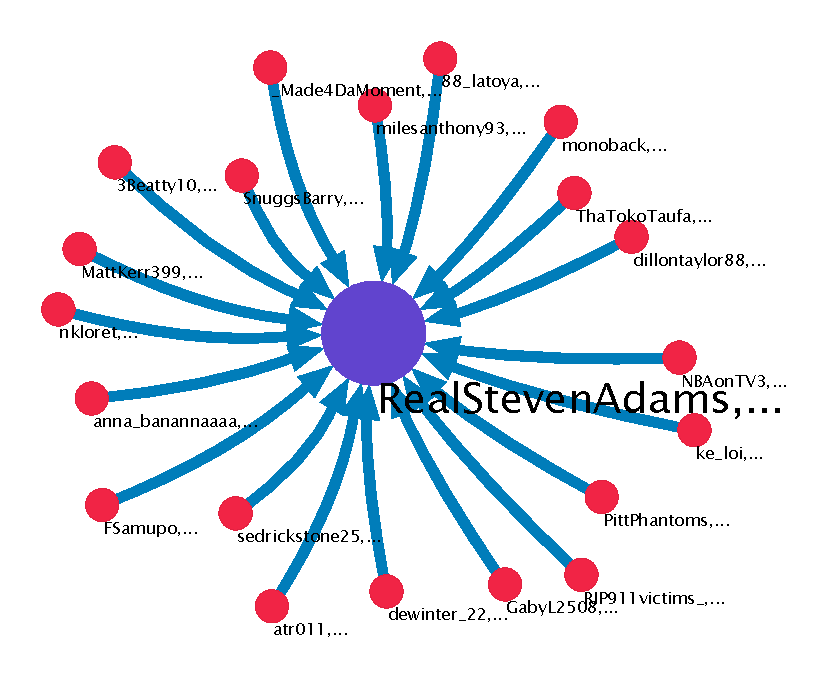
\includegraphics[width=300px]{Images/steven_adams_followers.pdf}
\caption{Followers of Steven Adams}
\label{fig:stevenadamsfollowers}
\end{center}
\end{figure}

% Unfortunately due to the limitations of the tool used, larger sets of data were not able to be loaded in this context. I feel that with more results, larger and connected communities would be evident through the follower and following connection on Twitter.

\subsection{Retweet Communities}

The second approach taken considers the communities formed on Twitter through retweeting of content. I consider two profiles to be connected if one retweets the other. This is ordered by the retweeter being connected to the original poster, respectively. Heavier weight is added to the connection if a user retweets posts from the user multiple times. As this retweet connection is richer, visualisations of communities formed are of more interesting structure. 

\begin{figure}[ht]
\centering
\begin{minipage}[b]{0.45\linewidth}
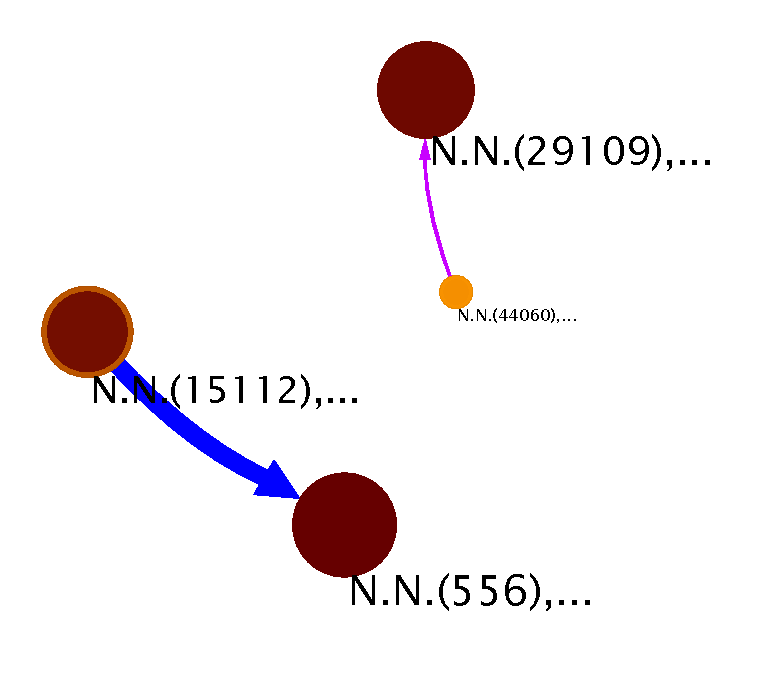
\includegraphics[scale=0.40]{Images/retweets_modules.pdf}
\caption{Retweet detected community modules}
\label{fig:minipage1}
\end{minipage}
\quad
\begin{minipage}[b]{0.45\linewidth}
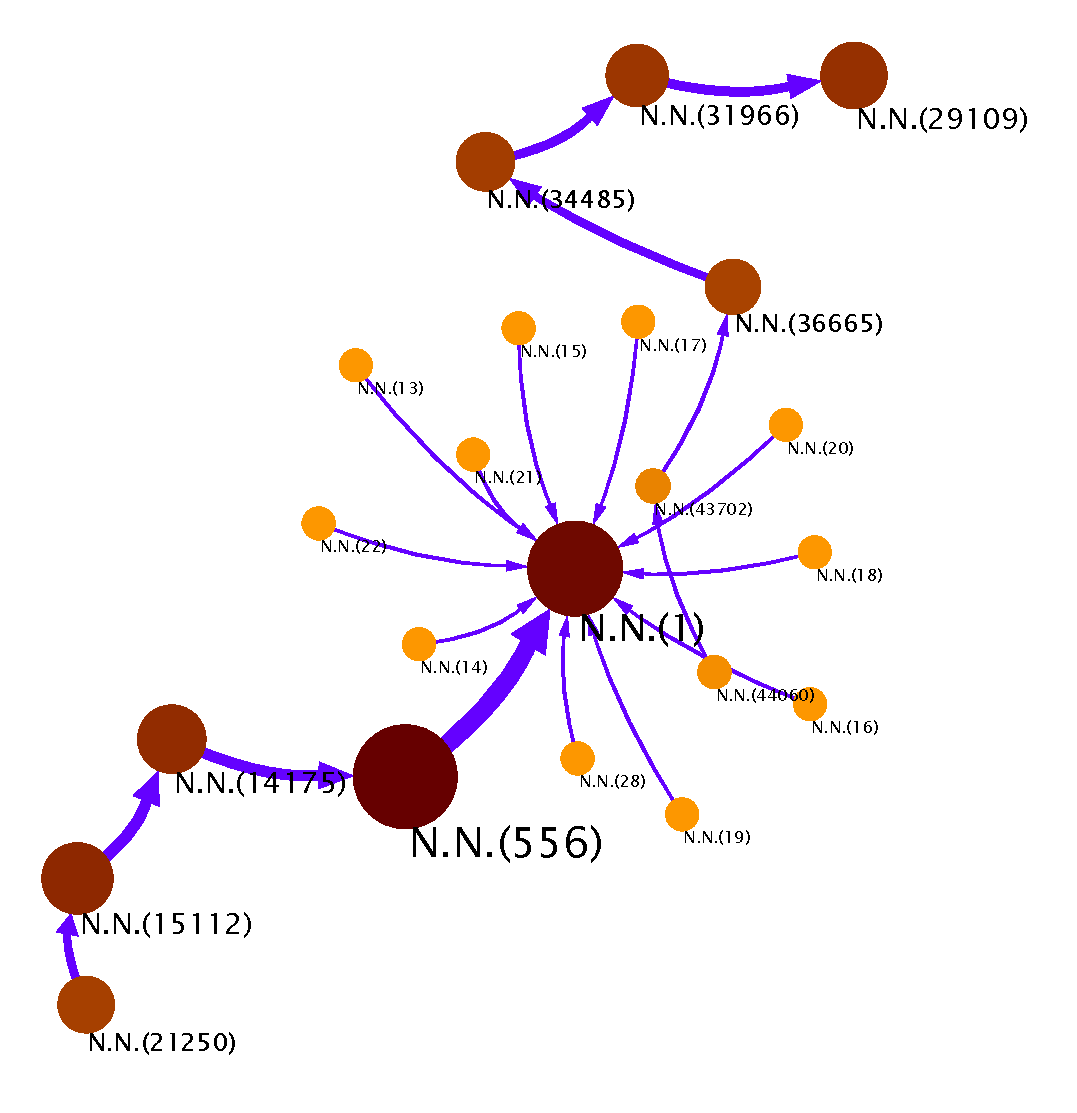
\includegraphics[scale=0.40]{Images/retweets_source_nodes.pdf}
\caption{Retweet source nodes}
\label{fig:minipage2}
\end{minipage}
\end{figure}

Unfortunately the MapGenerator tool did not allow for any entire set of profile and retweet data that was collected to be visualised in one piece. This is due to the extremely large quantity of nodes that are generated through the fetching of a single profile, and the entire collection of retweet or followers links associated with this profile. This largely reduced the use of current retweet communities, and the visualisation options for generating meaningful understanding of data collected, as arbitrary divisions in data necessary to be loaded into the tool introduce bias. Figures \ref{fig:minipage1} and \ref{fig:minipage2} are the retweet communities generated from the first quarter of one Twitter profile scraped. 

% as divisions in data were necessary to load into the tool introduce bias.

\subsection{Community Discussion}

The scrapers allowed for detection of communities for the two groups of followers and following, as well as detection of communities among retweeting circles. While the tools available certainly allowed for the detection of these communities, there is no way with the analysis tools currently provided to associate any real meaning with these groups. Future projects could assign meaning with the data that has been extracted - for example with sentiment or keyword classifying of tweet conversation topics for a profile. This would allow for meaningful classification of communities on Twitter, rather than simply grouping around profile names such as the grouping shown in Figure \ref{fig:stevenadamsfollowers}. This feature was left out of scope. Due to the large potential for extension of this community detection function, the policies ahead make assumptions on the classification of these groups being possible. 

%Positive outcomes of community detection - was able to group w.r.t to followers and following, as well as for retweeting communities.

%Limitations of community detection w.r.t. the connection between following/follower sets and the retweeter sets. Room left for development of components that are able to connect these sets. 

%Unfortunately limitations of the tools used to visualise and compute communities on Twitter, as well as scraping limitations resulted in 

%This investigation of community detection is not complete, and as such policies derived from community detection in this project are not entirely reflective of what I achieved. 

\subsection{Sentiment Analysis}

One avenue for enriching the community data would be to use sentiment-detection methods. Filip Dimitrievski's project was primarily focused on classifying social media posts based upon sentiment, and constructing policies based on this information. He was able to use data collected from the IHPScrape scrapers to classify tweets according to sentiment, with varying success with different classifiers such as Sentiment140\footnote{http://www.sentiment140.com/}. Although the classifier was not trained specifically to Twitter data and in the long run the approach was abandoned, this demonstrated the feasibility of such an approach. Future exploration of this is left to future work.

% Further exploration of this is left to future work, given that the project was not Artificial-Intelligence focused.

\section{Policy Examples and Discussion}

Reputation-inferring policies can be constructed from the data collected. Two exemplar policies are presented, which could be built as part of a system requiring reputation data related to a user's profile. These policies are applied in relation to a theoretical case study.

% I discuss 2 exemplar policies in particular which could be built as part of any system requiring reputation data related to a user's profile. I apply these policies in relation to a theoretical case study, that requires access policies based upon user reputation from an external source. 

\subsection{Case Study - Discussion Forum}

In order to introduce exemplar reputation policies, the concept of an interactive forum is used. This concept is inspired by Hendrikx at al. \cite{graft_paper}, where GRAft was applied to a social forum, using a pure reputation access control system. In this example, forum access control may be modified by restricting or granting additional rights to users based upon calculated reputation. Reputation is turned into access control rights by these policies.

As in the GRAft paper, I provide policy fragments, using Ruler\footnote{https://github.com/bobthecow/Ruler} to demonstrate how such a policy engine may operate. The following policy fragment restricts access based upon the impact factor of the given user, combined with the community that the individual is a part of. For example, on a computer science forum the administrator may only desire users with a significant social media impact to do with the engineering discipline to be able to post. In the example the calculated impact factor of the user is enfored to be greater than or equal to 1, and the computed community discipline is related to the current forum, in order to post. 

% Here I propose that the calculated impact factor of the user is greater than or equal to 1, and the computed community discipline is related to the current forum, in order to post. 

\begin{center}
 \textbf{Policy 1: Impact Factor and Community Participation}
\begin{verbatim} 
 $rb->logicalAnd(
  $rb['impact_factor'] -> greaterThanOrEqualTo(1),
  $rb['community_value'] -> in_array(['computer_science','engineering'])
 ) 
\end{verbatim}
\end{center}

Whereas for read-only rights, the person may only need to be part of the relevant discipline.

\begin{verbatim}
 $rb['community_value'] -> in_array(['computer_science','engineering'])
\end{verbatim}

On the same forum, administrator rights may be granted to consistently active users. Some evidence of consistent activity on social media might be required for effective administration of the site. In this exemplar policy, administration rights are granted to the user if their average monthly computed impact is greater than or equal to 3, and they are part of the computer science or engineering community. 

\begin{center}
 \textbf{Policy 2: Impact Factor, Community Participation and Temporal Consistency}
 \begin{verbatim}
   $rb->logicalAnd(
    $rb['temporal_impact_average'] -> greaterThanOrEqualTo(3),
    $rb['community_value'] -> in_array(['computer_science','engineering'])
  ) 
 \end{verbatim}
\end{center}


%Performance

%Resistance to Detection

%Logging


%Our definition of equivalent defines that 

%\section{Temporal Clustering}

%By looking at impact across a period of time, we are able to distinguish constant emitters from one-hit-wonders, who 

%\subsection{Correlation of Impact Factor vs Bucketed Impacts}

%\begin{figure}[h!]
%\centering
%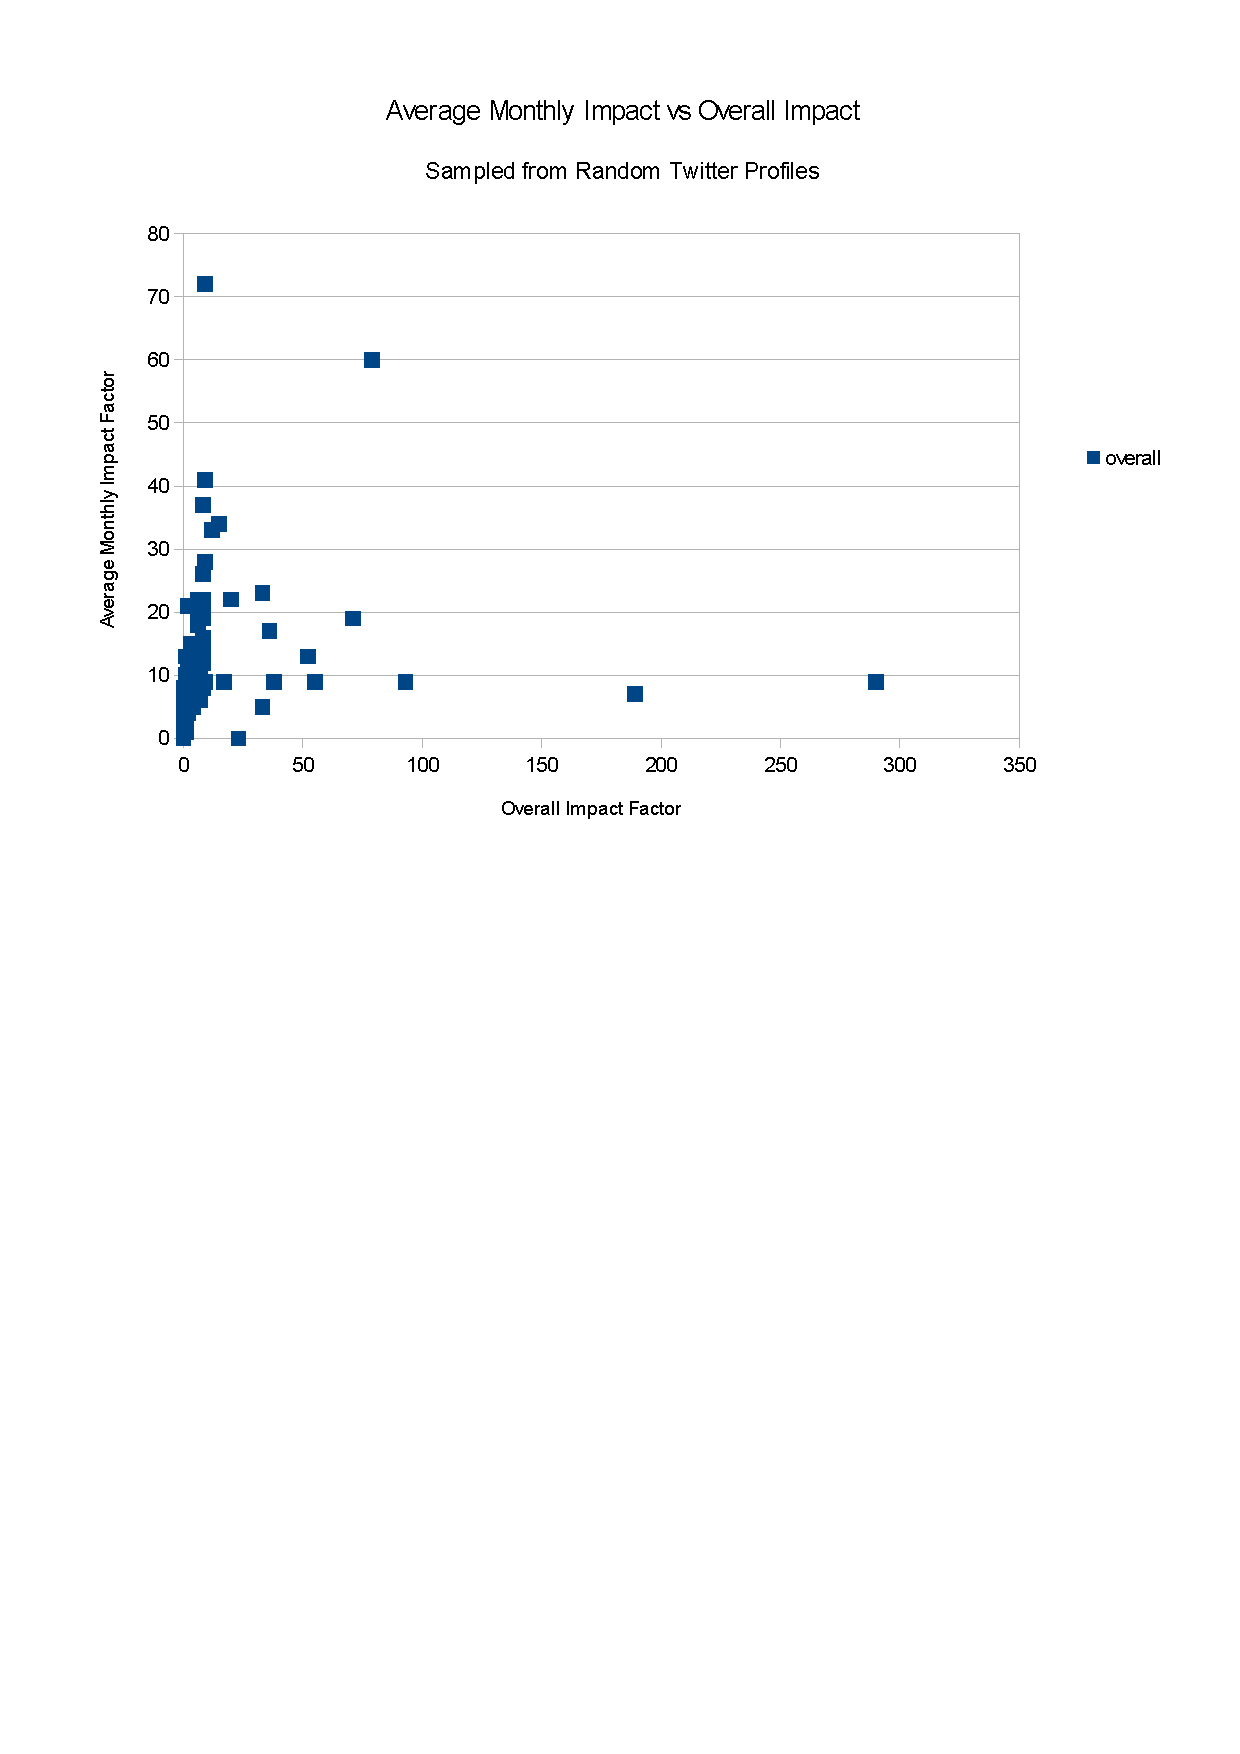
\includegraphics[width=400px]{Images/monthly_impact_vs_overallv2.pdf}
%\caption{Monthly Impact against Overall Impact}
%\end{figure}

%\begin{figure}[h!]
%\centering
%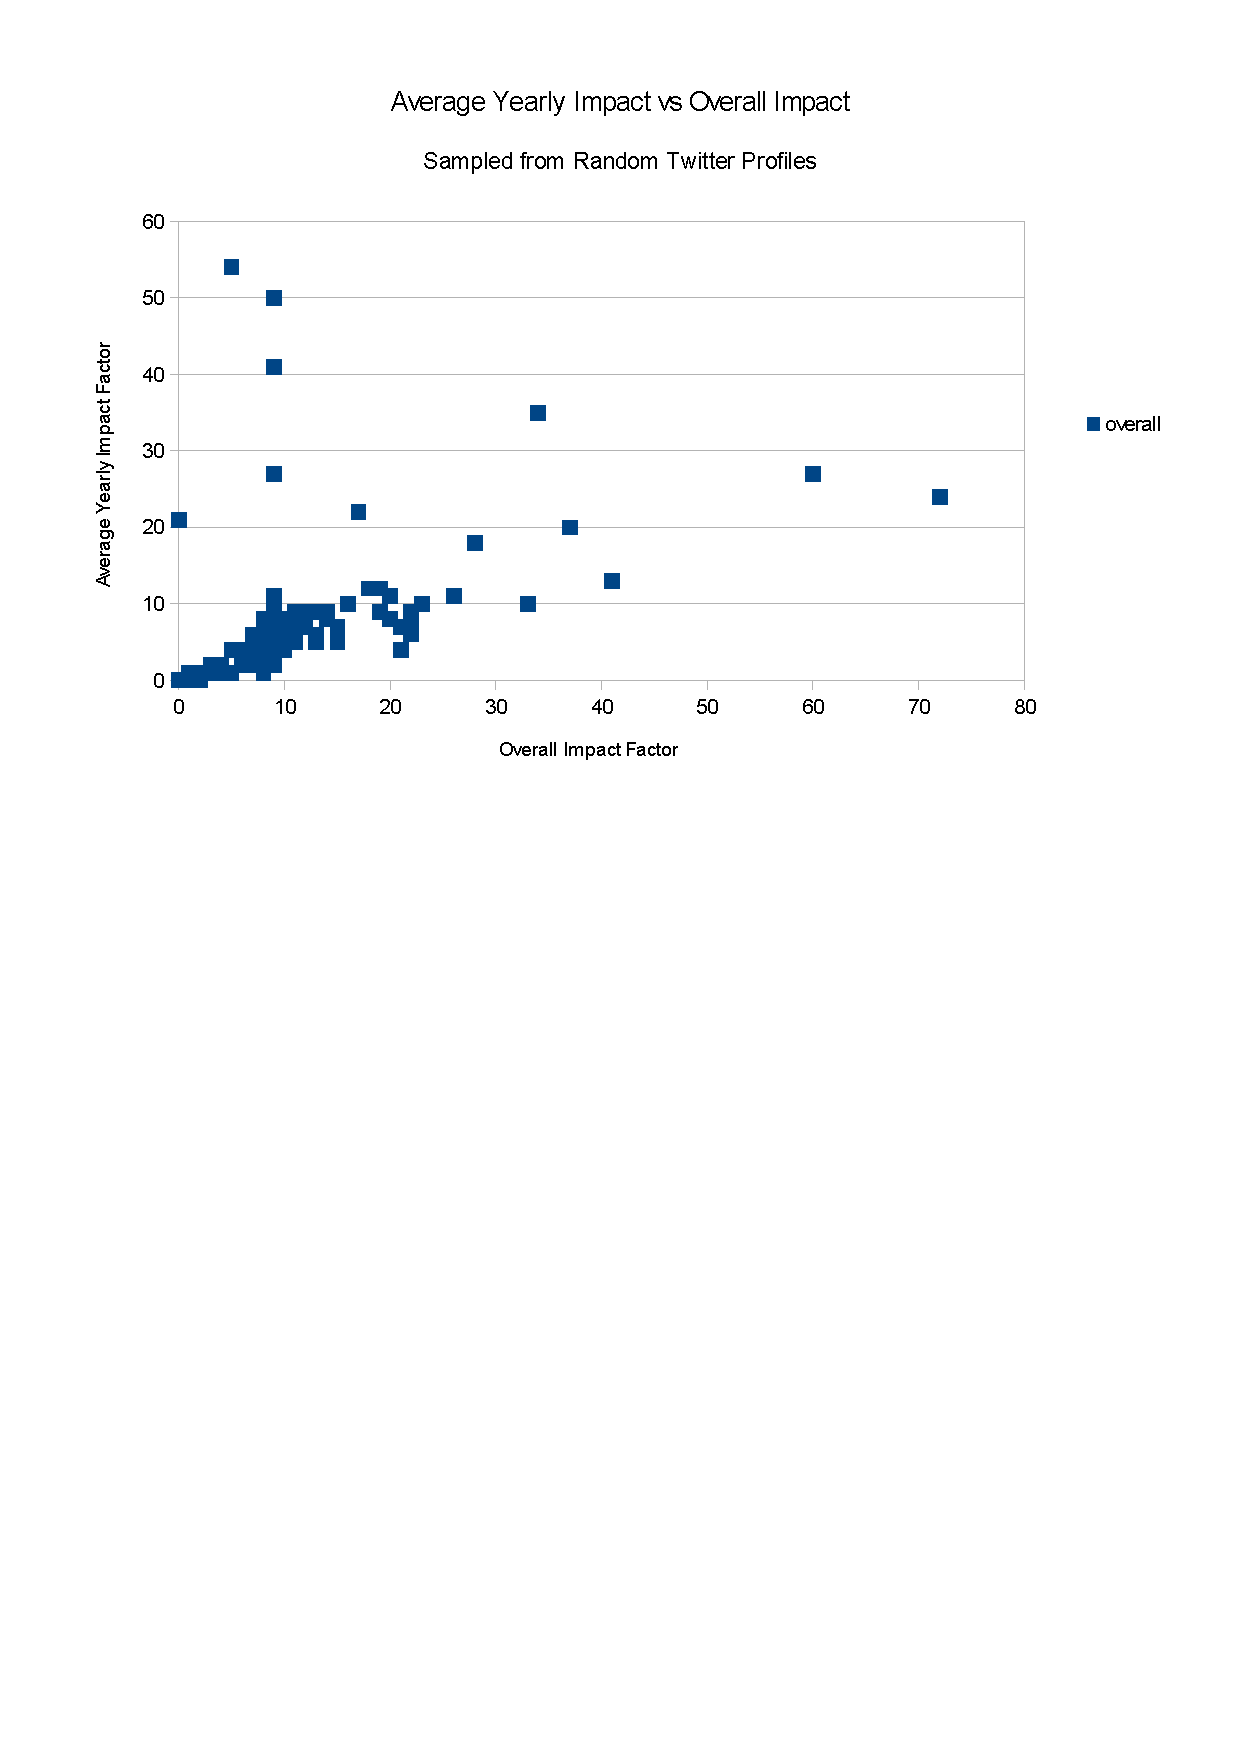
\includegraphics[width=400px]{Images/yearly_impact_vs_overallv2.pdf}
%\caption{Yearly Impact against Overall Impact}
%\end{figure}

%One strategy for inferring reputation information that I looked at was through temporal bucketing of impact factor, into days, months, and years. The figures below show the relationship between people's mean monthly calculated impact factor (i.e. by calculating a person's impact score for each month, and then averaging these values over the total number of months), and the individual's overall impact score. I infer that there is a weak relationship between average monthly impact and overall impact (Pearson's correlation coefficient of 0.273(3 s.f.)), and a stronger relationship between average yearly impact and overall impact (r=0.689(3 s.f.))\\

%\noindent What I believe this data shows is that the impact factor is favourable to individuals who are consistent on Twitter over time. 

%\subsection{Results of Monthly Bucketing}

%By applying the impact factor formula to individuals on a monthly basis, we are able to generate an impression of how regularly active a person is. The data also reveals how influential the person has been per month. This assists when comparing individuals who are consistently strongly influential (e.g. Barack Obama, companies such as instagram), with those who are popular for a limited period only. I looked at comparing different bucket sizes for this temporal aggregation. Days, months, and years were used as buckets, with monthly aggregation clearly showing the strongest and more interesting trends. 

%\begin{figure}[h!]
%\centering
%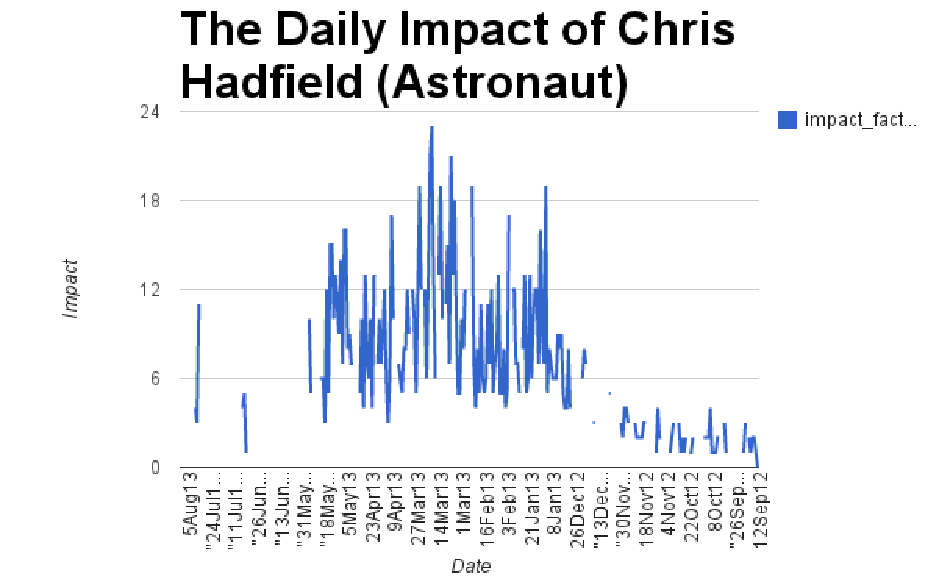
\includegraphics{Images/daily_impact_chris_hadfield.pdf}
%\caption{The Daily Impact of Chris Hadfield - Famous Astronaut}
%\end{figure}



%\begin{figure}[h!]
%\centering
%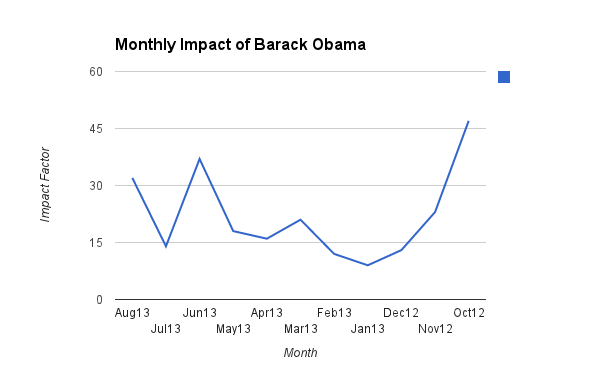
\includegraphics{Images/monthly_impact_barack_obama.png}
%\caption{The Monthly Impact of Barack Obama - President of USA (As if you didn't know that)}
%\end{figure}

%We can see that the daily and monthly impact trends follow roughly the same curve, which should be expected. The difference is due to the strictness of the impact factor formula in classifying someone as 'influential'. It is very difficult to get a value much above 1 on a daily basis, unless you are very frequently both making use of the social media, and having people respond to this activity. 


%\section{Monthly Bucketing of Impact}

%\section{Community Detection}

%\begin{description}
% \item [H2.] Sub-communities exist on Twitter, and we are able to detect these through scraping mechanisms.
%\end{description}



%One strategy for inferring reputation information that I looked at was through temporal bucketing of impact factor, into days, months, and years. The figures below show the relationship between people's mean monthly calculated impact factor (i.e. by calculating a person's impact score for each month, and then averaging these values over the total number of months), and the individual's overall impact score. I infer that there is a weak relationship between average monthly impact and overall impact (Pearson's correlation coefficient of 0.273(3 s.f.)), and a stronger relationship between average yearly impact and overall impact (r=0.689(3 s.f.))\\

%First present the use of retweets vs favourites on Twitter, and show that they are similar

%Next we look at impact factor of a person's retweets, pulled from the Hirsch-index formula. 

%Policies as an outcome of this, written using Ruler?